\documentclass[a4paper,11pt]{report}
%\pagestyle{headings}

% des paquetages indispensables, qui ajoutent des fonctionnalites
%\usepackage[latin1]{inputenc}
\usepackage[utf8]{inputenc}
\usepackage[french]{babel}
%\usepackage{lmodern}
\usepackage{amsmath,amssymb}
\usepackage{amsthm}
\usepackage{fullpage}
\usepackage{graphicx}
\usepackage{url}
\usepackage{xspace}
\usepackage{listings}
\usepackage{xcolor}
\usepackage{hyperref}
\usepackage{eurosym}

%%configuration de listings pour l'affichage du code
%\lstset{
%    language=C,
%    basicstyle=\ttfamily\small, %
%    identifierstyle=\color{red}, %
%    keywordstyle=\color{blue}, %
%    stringstyle=\color{black!60}, %
%    commentstyle=\it\color{black!50}, %
%    columns=flexible, %
%    tabsize=3, %
%    extendedchars=true, %
%    showspaces=false, %
%    showstringspaces=false, %
%    numbers=left, %
%    numberstyle=\tiny, %
%    breaklines=true, %
%    breakautoindent=true, %
%    captionpos=b,
%    frame=single
%}

% On fera des listes a puce et non a tiret.
\renewcommand{\FrenchLabelItem}{\textbullet}

\newtheorem{theoreme}{Th\'{e}or\`{e}me}
\newtheorem{definition}{D\'{e}finition}
\newtheorem{exercice}{Exercice}

\newcommand{\tab}{\hspace*{\parindent}}

%Definition de quelques commandes utiles en maths :

% R et N
\newcommand{\R}{\mathbb{R}}
\newcommand{\N}{\mathbb{N}}
\newcommand{\C}{\mathbb{C}}
% derive partielle et congruence
\newcommand{\drond}{\partial}
\newcommand{\congru}{\equiv}
% blocs parenthese, valeur absolue, norme, crochets, accolades
\newcommand{\abs}[1]{\left\lvert#1\right\rvert}
\newcommand{\norm}[1]{\left\lVert#1\right\lVert}
\newcommand{\braces}[1]{\left(#1\right)}
\newcommand{\croch}[1]{\left[#1\right]}
\newcommand{\cbraces}[1]{\left\{#1\right\}}
% blocs parties entieres superieur et inferieur
\newcommand{\entsup}[1]{\left\lceil#1\right\rceil}
\newcommand{\entinf}[1]{\left\lfloor#1\right\rfloor}





\title{Cannonball of RC cars\\User guide}
\author{Thibaut Coutelou, Benjamin Mugnier, Guillaume Perrin}
\date{\today}

\begin{document}
\maketitle
\tableofcontents
%\listoffigures

\setlength{\parskip}{3mm}

%\begin{figure}[!ht]
%\begin{center}
%\includegraphics[width=\textwidth]{img/acteurs}
%\caption{Acteurs}
%\label{acteurs}
%\end{center}
%\end{figure}

%Quick reminder of latex :
%part
%chapter
%section
%subsection
%subsubsection
%paragraph

%Don't forget : set tw=79

\chapter{Quick starter guide}

\section{What do I need ?}

You will need :
\begin{itemize}

    \item A radio-controlled car (we used the KYOSHO Scorpion XXL-VE).

    \item A webcam (we used the Logitech HD Pro Webcam C920).

    \item An Arduino (we used the Arduino UNO).

    \item A self-powered USB hub (without outlet).

    \item A Windows tablet, not running windows RT (we used the Lenovo ThinkPad
        tablet 2).

\end{itemize}

\section{How to plug ?}

Follow instructions on figure \ref{fig:wires}.

\begin{figure}[!ht]
\centering
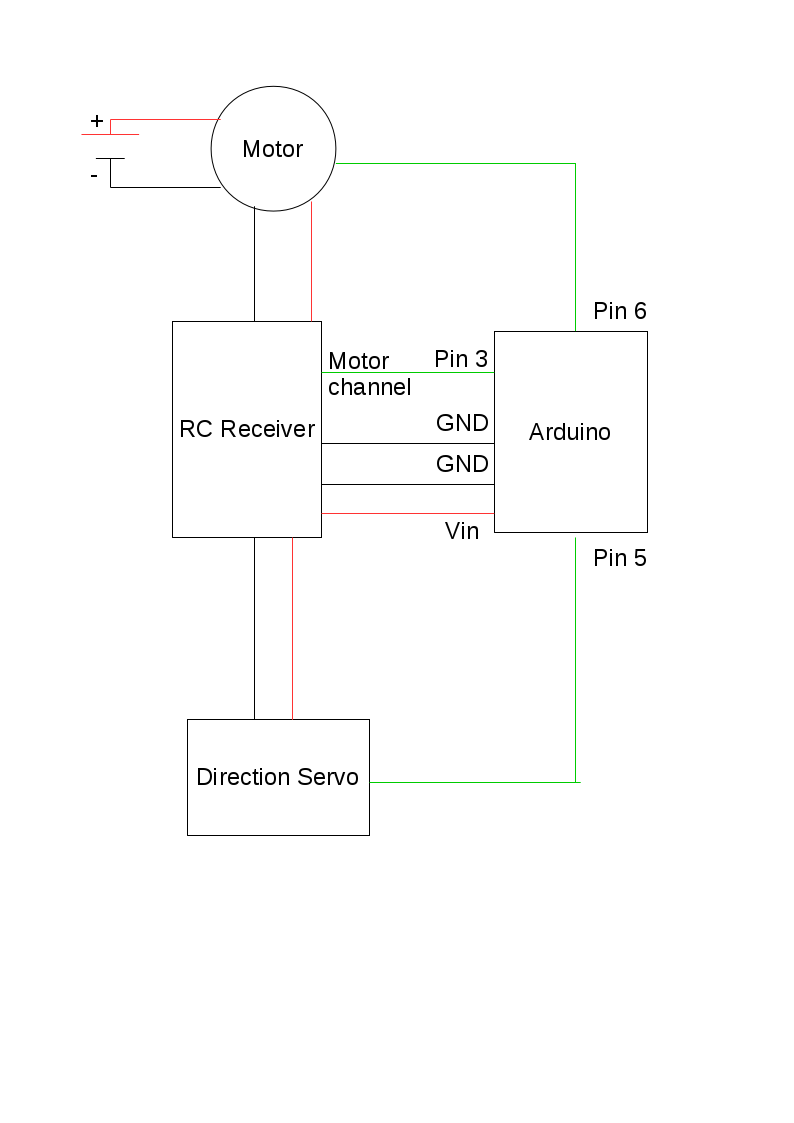
\includegraphics[scale=0.5]{img_static/wires}
\caption{How to plug}
\label{fig:wires}
\end{figure}

Be careful with the L led on the Arduino. If it turns on (orange), then the
Arduino will not compute any data from the tablet. You need to restart the
board using the Arduino reset button. This is in fact the emergency signal,
more informations on section~\ref{subsec:emergency}.

\section{How to flash the Arduino ?}

There are two ways to flash the Arduino, the first one (and the simple one) is
to use the Arduino
IDE\footnote{\url{http://arduino.cc/en/Main/Software\#toc1}}. After download,
open the project in it.

In order to flash the Arduino, you need to select the model in \texttt{Tools >
Board} and the serial port in \texttt{Tools > Serial Port}, this is likely
\texttt{COM3} or higher on Windows and \texttt{/dev/tty.usbmodem} on Unix systems.
You can now flash the file on Arduino using the shortcut \texttt{upload} or in
the menu \texttt{File > Upload}. You will see \texttt{Upload done} if everything
went well.

If you're interesting in the other method, please refer to \ref{sec:Flashing}.

\section{How to get markers ?}

Marker recognition is based on highly reliable markers (hrm) from the
arUco\footnote{\url{http://www.uco.es/investiga/grupos/ava/node/26}}
library.

Go to ressource folder, and print the needed markers. In this folder, you'll
also find yml files needed to run the executables with these markers.

If you're interested in designing new markers, please refer to the complete guide
section~\ref{sec:markers}.

\section{How to get metrics ?}

\subsection{Setup a MQTT server}

You need an MQTT server to get the data. We recommend
Mosquitto\footnote{\url{http://mosquitto.org/download/}} which is available for
every platform. Note that it's available on Debian (and derivatives) via a
simple \texttt{apt-get install mosquitto} and on OSX via \texttt{brew install
mosquitto}. For Windows, you need to download the server and then restart your
computer for the service to launch (or ask the service to launch manually),
this is really important.

Then, you need the tablet to be on the same network as the server. You can
either create a hotspot via the tablet or the server, or connect both to an
existing network. You need to tell the program the server's ip. Please refer
to section~\ref{sec:args}.

\subsection{Display metrics in HTML}

The metrics are retrieve through a Node
server\footnote{\url{http://nodejs.org/}}. You can download via \texttt{apt-get
install node} on Debian, \texttt{brew install node} on OSX and on the
\href{http://nodejs.org}{official website} on Windows. You also need a mongo
server that you can find on Debian via \texttt{apt-get install mongodb}, on OSX
via \texttt{brew install mongodb} and for Windows on the
\href{http://www.mongodb.org/downloads}{official
website}\footnote{\url{http://www.mongodb.org/downloads}}, you can launch the
mongodb sever via the command \texttt{mongo --dbpath </path/to/the/db>}.

After installing node, you need to install package dependencies by launching
the command \texttt{npm install} in the \emph{Mosquitto/subscriber} directory.
You also need to download \emph{Bootstrap 3} on the
\href{http://getbootstrap.com/}{official
website}\footnote{\url{http://getbootstrap.com}}, \emph{socket.io client} on
the \href{http://socket.io/download/}{official
website}\footnote{\url{http://socket.io/download/}} and \emph{Chart.js} on the
\href{http://www.chartjs.org/}{official
website}\footnote{\url{http://www.chartjs.org/}}

You are now able to launch the node server with the command \texttt{node
subscriber.js mqtt\_server\_address mqtt\_server\_port mongo\_port}. You can
now display the metrics in the web page \texttt{view.html}.

\section{How to launch the program ?}

The program is launched as usual by double-clicking the .exe, a console will
prompt.  For more informations on how to build the .exe, please refer to
section~\ref{sec:build}.

\subsection{Arguments needed}
\label{sec:args}

The executable needs several arguments. Otherwise, it will not launch and
prompt the program usage.
The program needs :

\begin{itemize}
    \item Path to dictionnary.yml, see~\ref{subsec:dic}.
    \item Path to intrinsics.yml, see~\ref{subsec:cam}.
    \item Marker size (in meters).
    \item The MQTT server IP for getting metrics.
    \item The Arduino serial port, should be something like 'COM5'.
    \item The mode to run (AI). Should be \emph{rabbit} to follow a marker, or
        \emph{cannon} for race mode.
    \item Additional parameters for AI
\end{itemize}

\subsubsection{Additional parameters AI}

For the \emph{rabbit} AI, you have to add one parameter, the marker identifier
to follow.

For the \emph{cannon}AII, you have to add one parameter, the file containing
markers identifier which form the doors. See section \ref{subsec:doorsfile} to
know how to create the file.

\chapter{User guide}

\section{Building}
\label{sec:build}

\subsection{Libraries}

First, you need to install OpenCV\footnote{\url{http://opencv.org/}} 2.4.8 and
Mosquittopp\footnote{\url{http://mosquitto.org/download/}}.

\subsection{Visual Studio 12}

We used Visual Studio 12 to develop and build the program.

Open Visual Studio, create a new project, add all the \texttt{.h} and
\texttt{.cpp} files.

Open the project properties, go to Project, Properties, C/C++, general,
additional include directories. Add the path to the include directories of
mosquittopp and opencv.

Open the project properties, go to Project, Properties, linker, general,
additional library directories. Add the path to the libraries directories of
mosquittopp and OpenCV (directory with all the \texttt{.lib} files).

Open the project properties, go to Project, Properties, linker, general, input,
additional dependencies. Add all the \texttt[.lib] files of mosquittopp and
OpenCV.

You should now be able to build the program (Ctrl-Shift-B).

Copy all the \texttt{.dll} files of mosquittopp and OpenCV to the directory of
the executable.

Create a shortcut to the .exe, edit it to set the arguments.

You should now be able to run the program !

\section{Flashing}
\label{sec:Flashing} %Need in user quick guide->flash arduino

You can flash the Arduino using Arduino IDE as described in the quick start
guide. However, there is another way to do it via console.

You can use Ino Tool\footnote{\url{http://inotool.org/}}. You'll be then able
to compile using the provided MakeFiles.

Do not forget to change the value of ARDUINO\_MODEL in the MakeFile. To find
which Arduino model you're using, just type ino list-models in a terminal.

If you don't want to use the MakeFiles, here is a simple guide to compile via
command line with Ino :
\begin{itemize}
    \item To build, use \texttt{ino build -m 'model'}
    \item Then you need to upload on the board, use \texttt{ino upload -m 'model'}
    \item If you want to remove generated files, use \texttt{ino clean}
\end{itemize}

\subsection{Debugging serial communications}

You can use Arduino IDE to display and/or write serial data, just click on the
serial monitor icon (upper right) to display a terminal.

If you prefer to use ino, you need first to install picocom, then run ino
serial.

\section{Plugging}
To properly plug, please see figure~\ref{fig:wires}.

\subsection{Supply}
Circuit supply is based on the motor, which itself is plugged to the
battery. So the circuit is supplied once the motor is turned on, and supply the
RC reciver, which act as a energy spreader.

That's why you need to plug the Arduino VIN pin to the RC receiver to grab
energy. Don't forget to also plug the grounds.

Please note that the VIN in Arduino is not truly a IN signal. The Arduino can
also provide supply through this pin if the board is supplied elsewhere. For
instance, if you plug the USB cable and you don't power on the motor, the
Arduino board will provide energy via the VIN port (leeching from USB), meaning
the circuit will be supplied. But this is not sufficient to supply the whole
circuit (the motor will start beeping, meaning it doesn't have enough energy to
run). This is really important and should be avoided.

Don't forget to plug the motor and the steering servo to the receiver for
supply. Do not plug the signal (white) wires. You can plug supply wires where
you want on the receiver.

Also to avoid any problem, you should first plug the Arduino via VIN and only
after via USB, not the other way.

\subsection{Control}

Control wires are displayed in green on the schema. They are white wires on the
board.

Steering signal PIN should be connected to the PIN 5.
Propulsion signal PIN should be connected to the PIN 6.

Be careful when plugging these PIN. The car should be placed on a box, so that
the wheels can spin freely.

\subsubsection{Emergency signal}
\label{subsec:emergency}

Finally, plug the PIN 3 on the motor signal on the receiver. This is the
emergency signal. If you press the motor button on the radio, the orange led on
the Arduino will turn on, meaning that the car is in emergency state and will not
process the data received by the tablet. To go back to normal mode (and turn
off the led), you need to press the reset button on the Arduino. Please note
that the car will also go in emergency mode if it didn't receive data for 1
second.

\section{Markers}
\label{sec:markers}

\subsection{Camera calibration}
\label{subsec:cam}

First, you need to calibrate the camera. In order to do that, \begin{itemize}

    \item Generate a board of markers with \texttt{aruco\_create\_board 4:5
        boardImageCalibration.png boardConfigurationCalibration.yml}.

    \item Print the png image. Mesure in meters the size of a marker.

    \item Convert the board configuration file from pixel to meters with
        \texttt{aruco\_boar\_pix2meters boardConfigurationCalibration.yml <size
        of marker in meters> boardConfigurationCalibrationMeters.yml}

    \item Calibrate the camera with \texttt{aruco\_calibration live
        boardConfigurationCalibrationMeters.yml cameraParams.yml}

\end{itemize}

\subsection{Creating hrm markers}
\label{subsec:dic}

You now need to create markers : \begin{itemize}

    \item Generate a dictionary of hrm markers with
        \texttt{aruco\_hrm\_create\_dictionary dict.yml <size of the
        dictionary> <marker size>}

    \item Generate the board with \texttt{aruco\_hrm\_create\_board dict.yml
        board.yml board.png height width}

    \item Print the board.

\end{itemize}

\subsection{Configuration file for CannonBall AI}
\label{subsec:doorsfile}

The CannonBall AI requires a configuration in order to know marker identifiers
which make up the doors. The file has the following format : it contains a
sequel of identifiers order by the way of the track, left marker first, right
marker after, separate by spaces (space or carriage return).

\section{Implementing new artificial intelligence}

The application is designed to provide an easy way to add a new artificial
intelligence.

It is based on the strategy pattern. You need to create a new cpp class
(preferably named AImy\_ia\_name) which will implement the AI class.
\begin{verbatim}
    class AImy_ia_name : public AI
\end{verbatim}
Then, because it implements AI, you need to override \texttt{getCommand} (in
\emph{cpp} this kind of function is called pure virtual, virtual meaning
undefined and pure meaning it has to be redifined in every sub class).
\begin{verbatim}
	virtual void getCommand(vector<aruco::Marker>* TheMarkers, int* steering,
    int* throttle, int width);
\end{verbatim}
\texttt{getCommand} will change steering and throttle values. You can use the marker
vector (which represents all markers recognized for this frame) to make a
decision.

Don't forget to add your new AI as program parameters. You'll need to :
\begin{itemize}
    \item Add your AI in the AI enumeration called \emph{Runmode} at the beginning of the
        program.
    \item Add your AI in \texttt{readParams} to change the runmode according to you AI.
    \item Add your AI in choose\_run\_mode to instantiate it properly.
\end{itemize}
You should then be able to pass your AI as argument the same way as rabbit or
cannon using argument 6.

\section{Android}

The Android project can be find in the \emph{CannonBallDroid} directory.

In order to open and compile it, you must have Android
SDK\footnote{\url{http://developer.android.com/sdk/index.html}}.
You must have a tablet or phone on Android 4.0 or later to run it.
The project requires two libraries OpenCV, that you can download on the
official website and Android Serial
Library\footnote{\url{https://github.com/mik3y/usb-serial-for-android}}.

The Android port has been initialized, but a lot of code is commented, you
need to adapt this code for Android in order to finish the port on this
platform.

\end{document}
